\begin{columns}[totalwidth=.85\linewidth]
	\column{\textwidth}
	\vspace{-10mm}
		\begin{boxnote}
			\textbf{高分子材料でマルチマテリアル化 $\Leftrightarrow$ 高い比強度の有効利用}
			\begin{itemize}
				\item {\color{red} 「接着接合」}への高分子の利用
					\begin{itemize}
						\normalsize
						\item 柔らかさを生かした{\color{red} 「弾性接着接合」}
						\item 耐久性、可逆性に優れた\alert{ゴム材料に注目}
					\end{itemize}
				\item {\color{blue}耐久性が不明確}
					\begin{itemize}
						\normalsize
						\item とくに疲労破壊に対して
					\end{itemize}
			\end{itemize}
		\end{boxnote}

		\begin{itembox}[l]{ヒステリシスと破壊靭性}
			\begin{columns}[totalwidth=\linewidth]
				\column{.75\textwidth}
					\begin{itemize}
						\item 力学的ヒステリシス
						\begin{itemize}
							\normalsize
							\item
							\textcolor{blue}{loading} 時に比べて、\textcolor{red}{Unloading} 時の応力が低下
							\item
							ヒステリシスロス:変形時のエネルギー散逸
						\end{itemize}
						\item 破壊靭性との関係
						\begin{itemize}
							\normalsize
							\item
							Andrews 理論:ヒステリシスロスの重要性が指摘
						\end{itemize}
					\end{itemize}
				\column{.25\textwidth}
					\centering
					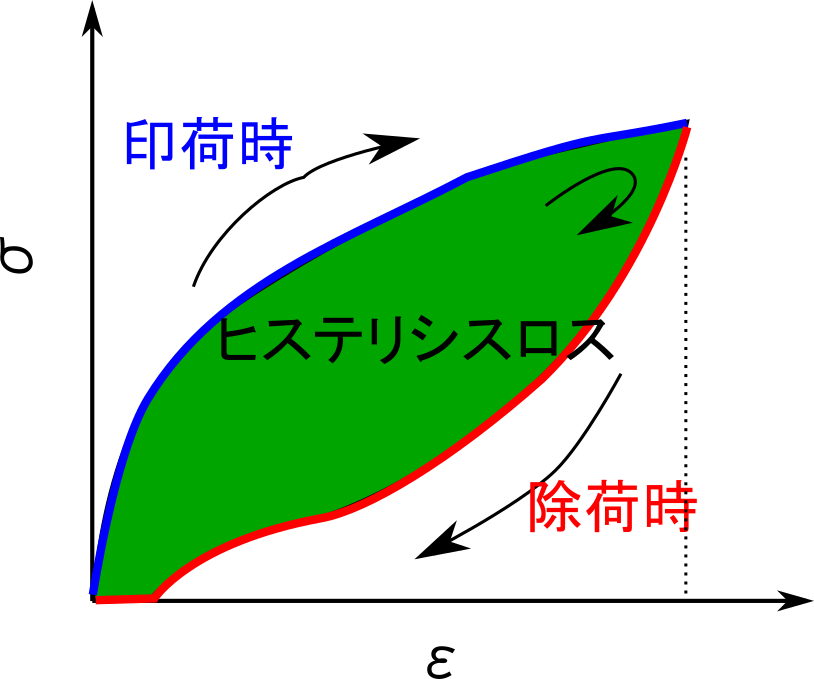
\includegraphics[width=\textwidth]{hysteresis_curve.png}
				\end{columns}
		\end{itembox}

		\begin{itembox}[l]{Andrews 理論\cite{andrews}}
			\begin{columns}[totalwidth=\textwidth]
				\column{.8\textwidth}
					クラックの微小進展時に、
					\begin{itemize}
						\item
						\textcolor{blue}{Loading 場}と\textcolor{red}{Unloading 場}のひずみエネルギーの差
						\item
						全体の変形に要したエネルギーの多くを\textcolor{red}{散逸}
						\item
						鎖の破断へのエネルギーが低減 $\Rightarrow$ \alert{強靭さの起源。}
					\end{itemize}	
				\column{.2\textwidth}
					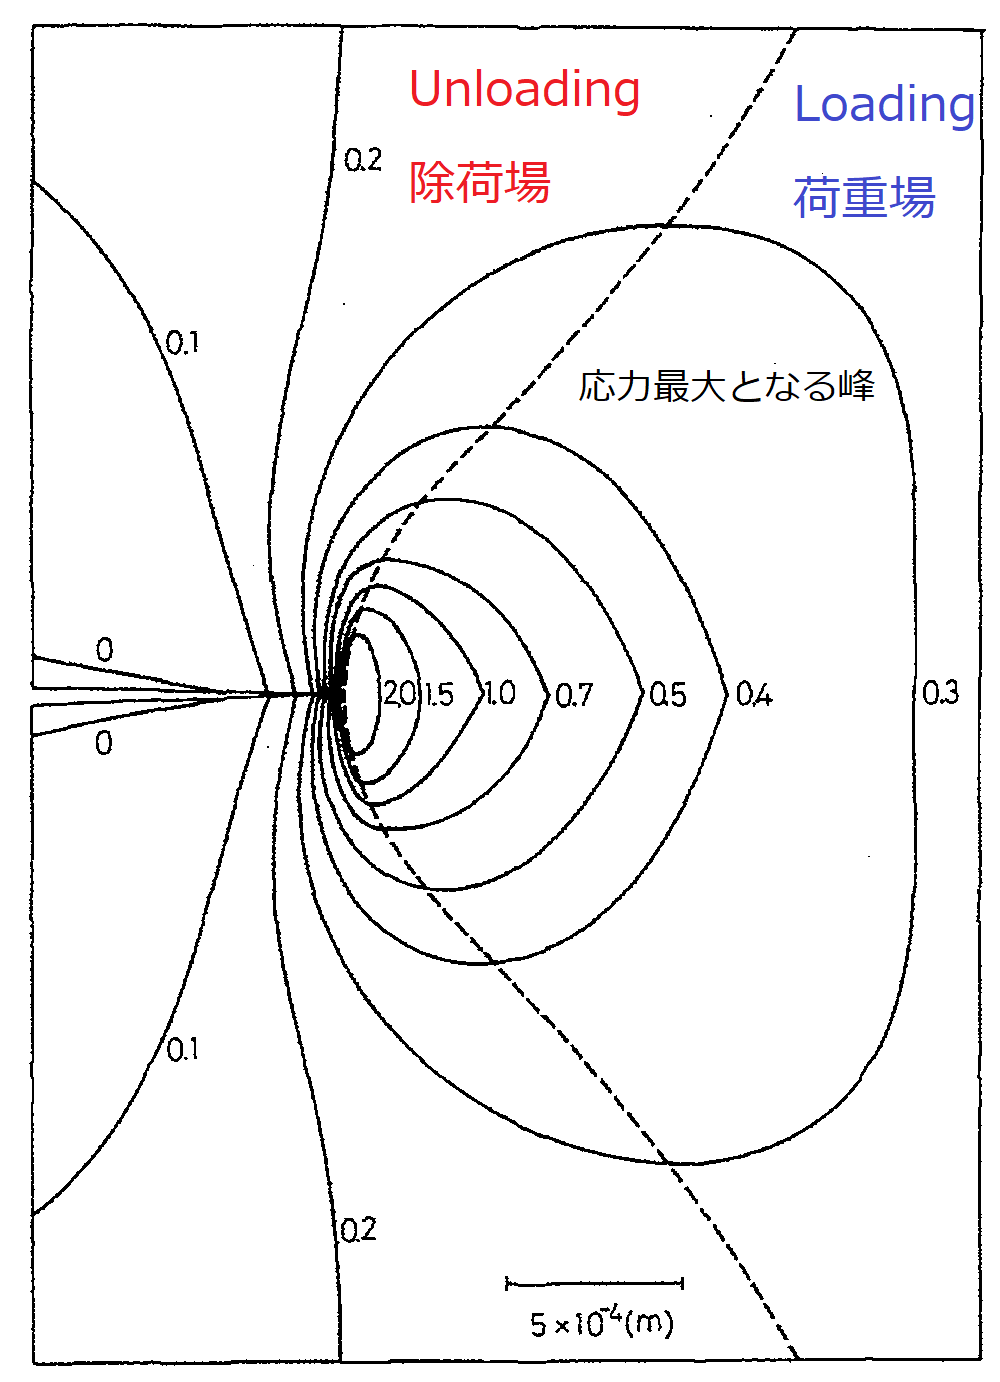
\includegraphics[width=.85\textwidth]{crack.png}     
			\end{columns}
		\end{itembox}

		\begin{itembox}[l]{ゴムの破断強度の時間温度依存}
			\begin{columns}[totalwidth=\textwidth]
				\column{.5\textwidth}
					\alert{粘弾性極限}\cite{lake}(高温・低速)
				\column{.5\textwidth}
					変形速度、温度\cite{smith} で\alert{破壊包絡線}
			\end{columns}
			\begin{columns}[totalwidth=\textwidth]
				\column{.5\textwidth}
					\centering
					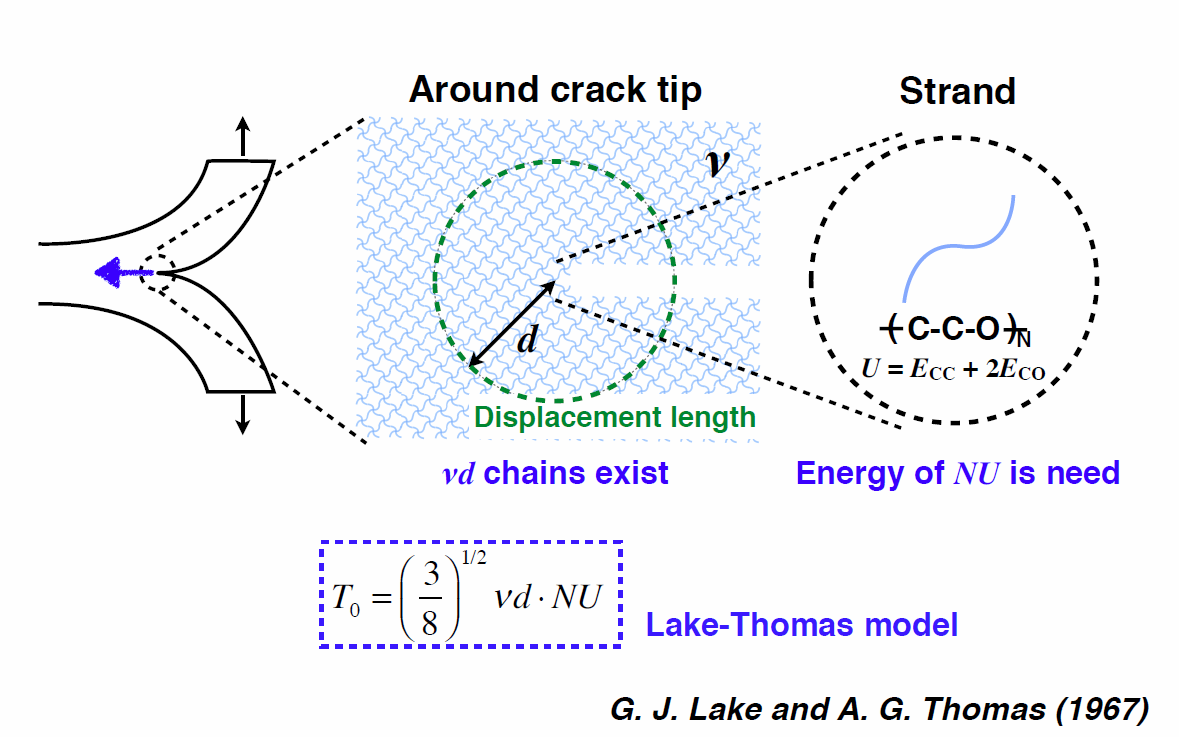
\includegraphics[width=.8\textwidth]{Lake_Thomas.png}
				\column{.25\textwidth}
					\centering
					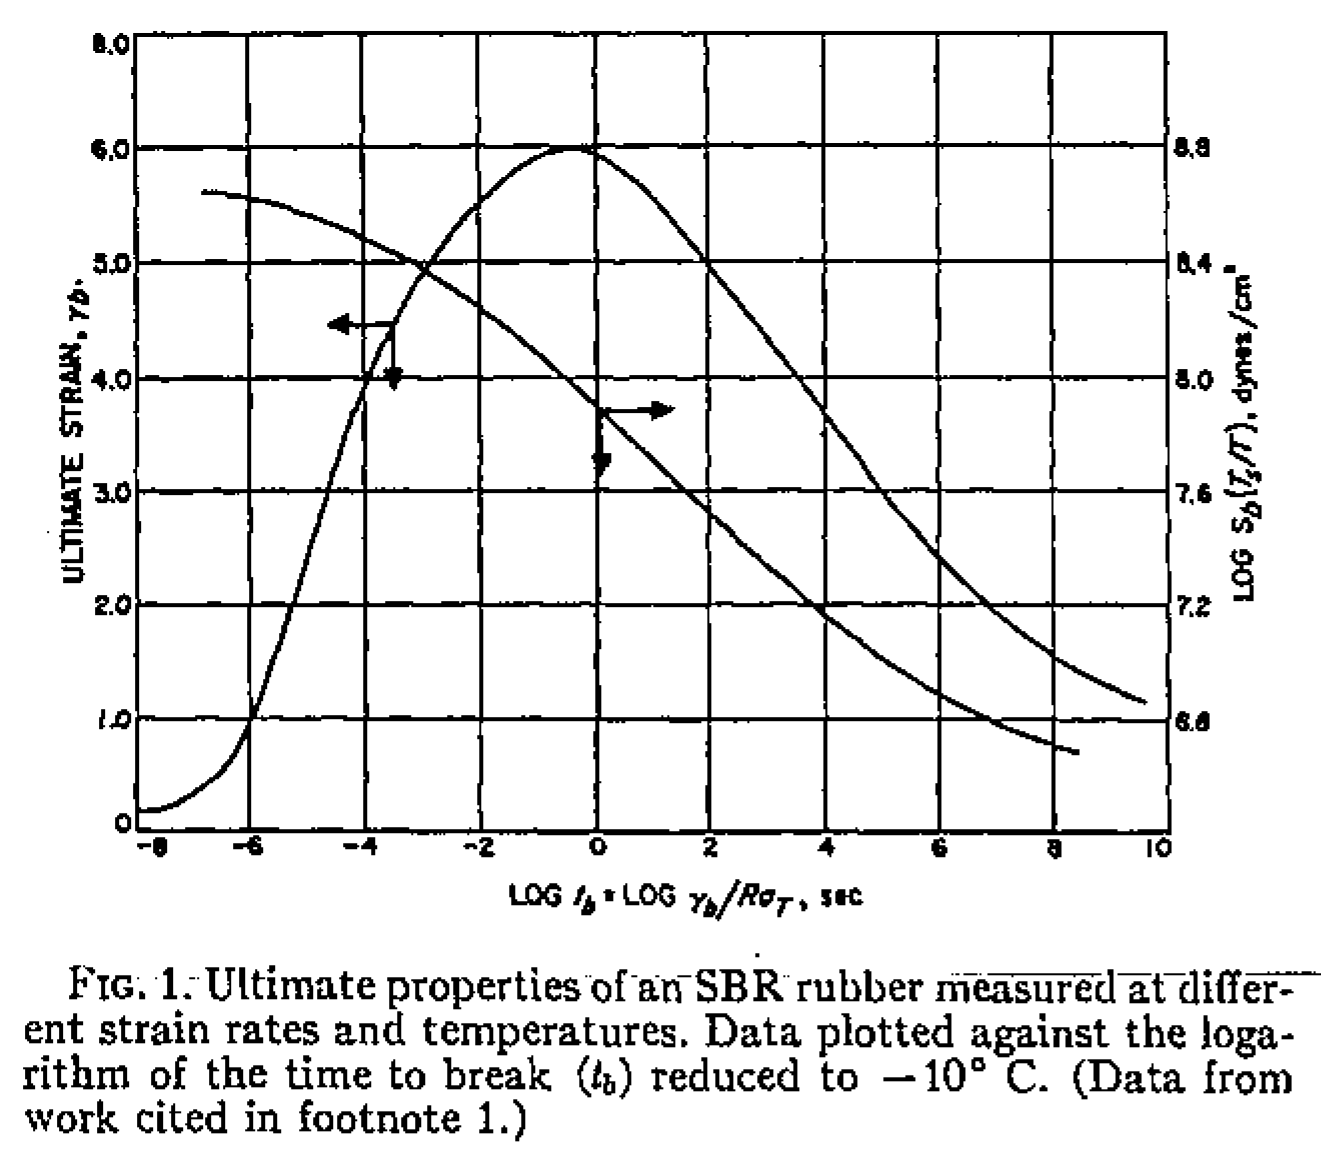
\includegraphics[width=.9\textwidth]{Time_Temp_2.png}
				\column{.25\textwidth}
					\centering
					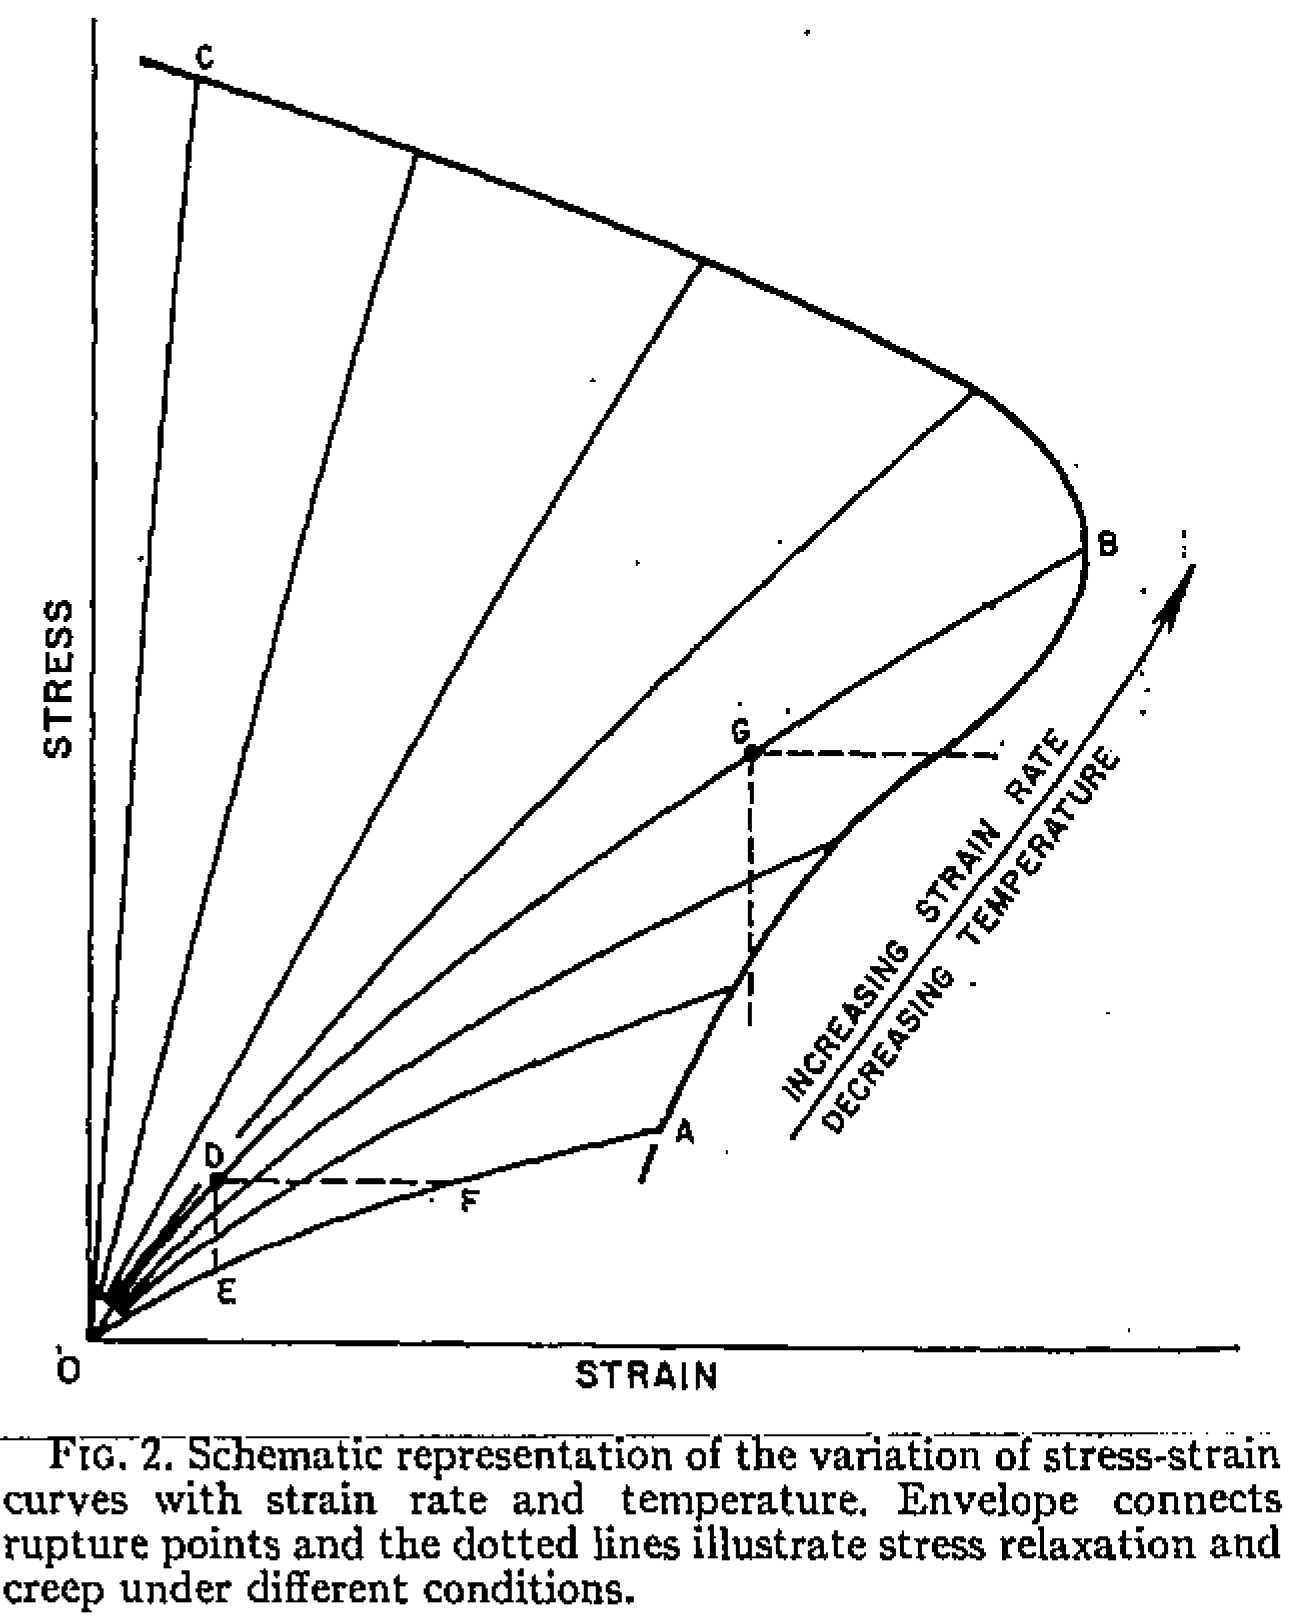
\includegraphics[width=.7\textwidth]{Time_Temp_3.png}
			\end{columns}
		\end{itembox}

		\begin{itembox}[l]{架橋点の環境とランダムな接続性\cite{flory}}
			\begin{columns}[totalwidth=\textwidth]
				\column{.35\textwidth}
				\centering
					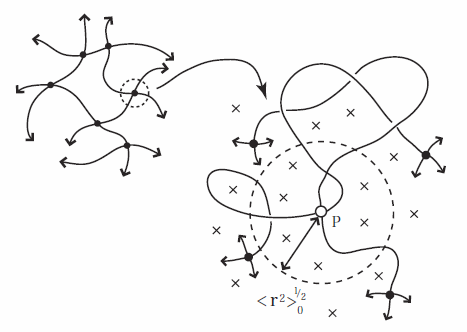
\includegraphics[width=.8\textwidth]{JP_vicinity.png}

					\small
					架橋点は\alert{多数のストランド}に\\囲まれている。
				\column{.4\textwidth}
					\begin{itemize}
						\item 接続性を不均一に
							% \begin{itemize}
							%     \item 接続に\alert{位置依存性}
							% \end{itemize}
						\item 巨視的な変形後
							\begin{itemize}
								\normalsize
								\item \alert{結節点のゆらぎが\\不均一}
								\item 多様な緩和モード
								% \item \alert{緩和の長時間化?}
							\item \alert{Phantom Network の\\諸特性が発現}
							\end{itemize}
					\end{itemize}
				\column{.25\textwidth}
					\centering
					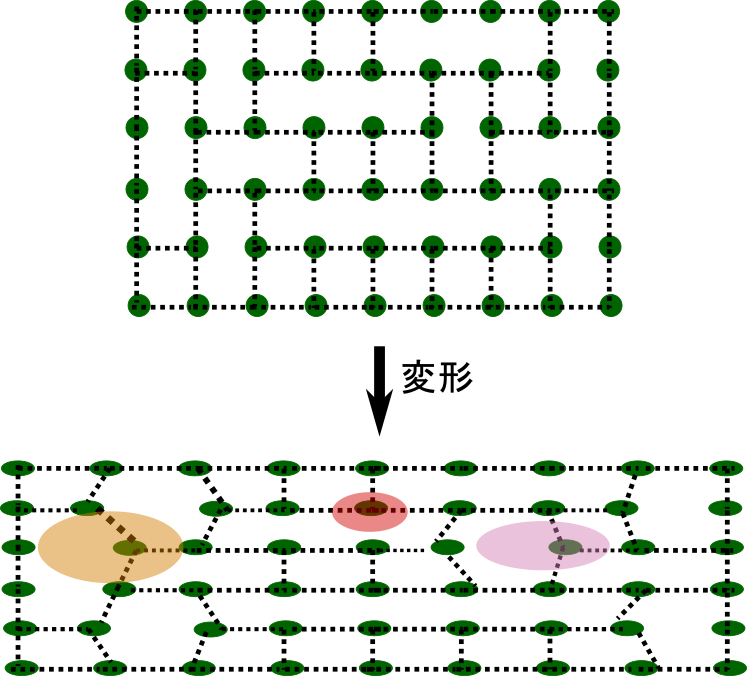
\includegraphics[width=\textwidth]{random_NW.png}
			\end{columns}
		\end{itembox}
\end{columns}